% Introdução

\documentclass[_ArquivoPrincipal.tex]{subfiles}

\begin{document}

%==================================================================================================
\chapter{Estado Da Arte}
%==================================================================================================
	
No presente capítulo serão abordados os principais temas relacionados à problemas de Interação Fluido-Estrutura (IFE), tendo como ênfase os modos de turbulência. Serão destacados os principais métodos de cálculos envolvendo a dinâmica das estruturas computacional (\ref{CSD}), a dinâmica dos fluidos computacional (\ref{CFD}) e alguns modelos de turbulências (\ref{MT}).

%==================================================================================================
\section{Dinâmica Das Estruturas Computacional} \label{CSD}
%==================================================================================================

A mecânica dos sólidos visa a determinação de parâmetros referentes à elementos estruturais sujeitos a solicitações externas, tais como tensões e deformações, ou forças e deslocamentos de determinados pontos dos mesmos. Para isso são desenvolvidos diversos métodos com a finalidade de melhor descrever o comportamento das estruturas, como o Método dos Elementos Finitos (MEF), que se apresenta como a ferramenta computacional mais amplamente utilizada para esse fim.

Nesse sentido vale ressaltar os trabalhos de \citeonline{hughes1981nonlinear, argyris1982excursion, ibrahimbegovic2002role, pimenta2004fully, battini2006choice} e \citeonline{pimenta2008exact}, que realizaram análises através do MEF Corrotacional, que se trata de uma formulação onde os deslocamentos e rotações dos elementos são os parâmetros principais da análise.

No entanto a utilização de uma análise que considera tais parâmetros nodais só se mostra eficiente ao se estudar estruturas que desenvolvem pequenos deslocamentos e deformações. Isso deve-se ao fato de essa abordagem utilizar rotações finitas como parâmetros nodais, o que pode gerar controversas em problemas envolvendo grandes rotações, uma vez que não há comutatividade entre essas grandezas. Ainda observa-se que a avaliação dinâmica de estruturas reticuladas se torna problemática, do ponto de vista da conservação de energia, além da matriz de massa ser variável, tornando o processo de integração temporal muito complexo \cite{sanches2013unconstrained}.

Com isso, vale ressaltar os trabalhos de \citeonline{coda2004simple, coda2007alternative, coda2010improved, coda2009two, coda2009unconstrained} e \citeonline{carrazedo2010alternative} que utilizam de forma bem-sucedida o MEF Posicional para análise de estruturas reticuladas e de cascas aplicadas à grandes deslocamentos. Este método se diferencia dos demais ao considerar as posições nodais, obtidas a partir de vetores indeformados, como parâmetros de análise, facilitando o cálculo de efeitos de não-linearidade geométrica.

\citeonline{sanches2013unconstrained} apresentaram uma aplicação do método dos elementos finitos posicional em elementos de cascas e constataram a presença de uma matriz de massa constante, o que possibilita a utilização de métodos de integração temporal, como o método de Newmark $\beta$, conservando, assim, o momento linear e angular em análises dinâmicas. Além disso, esse trabalho também analisou problemas envolvendo IFE, obtendo resultados favoráveis, indicando a boa aplicação desse método em problemas dessa natureza.

No âmbito da IFE, destaca-se a necessidade dessa consideração, uma vez que são observadas aplicações como, por exemplo, grandes amplitudes de deslocamentos, como \textit{flutter}, aplicações biomecânicas, estruturas infláveis \cite{karagiozis2011computational}, simulações de turbinas \cite{bazilevs20113d}, dentre outras.

%==================================================================================================
\section{Dinâmica Dos Fluidos Computacional} \label{CFD}
%==================================================================================================

Ao contrário de problemas envolvendo elementos sólidos, que possuem um estado inicial bem definido, os fluidos, em especial os Newtonianos, não o possuem, uma vez que não incapazes de resistir à tensões desviadoras, deformando-se, assim, indefinidamente quando sujeitos à essas tensões. Dessa forma, torna-se apropriada a utilização de uma descrição Euleriana para descrever os fluidos, em que os parâmetros nodais são principalmente as velocidades do mesmo \cite{fernandes2020tecnica}.

Em geral, problemas envolvendo Dinâmica dos Sólidos (\textit{Computational Solid Dynamics} - CSD) partem do princípio da estacionariedade de energias, buscando a determinação do ponto em que a energia do sistema seja mínima. Esses métodos apresentam a particularidade de surgir um sistema de equações com uma matriz simétrica e, em alguns casos, de vetores cujas componentes possuem significado físico. Porém, em problemas que envolvem a Dinâmica dos Fluidos (\textit{Computational Fluid Dynamics} - CFD), o sistema de equações possui uma matriz, na maioria dos casos, assimétrica, devido à presença de termos convectivos nas equações governantes \cite{bazilevs2013computational,brooks1982streamline}.

Nesse sentido, são desenvolvidos novos métodos, em busca de uma solução mais representativa com uma malha menos refinada. Dentre os principais desenvolvidos, vale mencionar o \textit{Streamline-Upwind/Petrov-Galerkin} (SUPG) \cite{brooks1982streamline}, \textit{Galerkin Least-Squares} (GLS) \cite{hughes1989new,tezduyar1991stabilized}, \textit{Subgrid Scales} (SGS) e \cite{hughes1995multiscale}.

Um campo que vale destacar na CFD é o que estuda os fenômenos de turbulência, uma vez que esses fenômenos podem se apresentar nas mais variadas escalas, sendo necessário a geração de uma malha muito refinada para detectar a formação dos vórtices, o que ocasiona um aumento radical no custo computacional da análise. Assim, são desenvolvidas novas técnicas afim de se obter melhores resultados, sem que haja um grande aumento no volume de cálculos. Dentre esses métodos destacam-se os métodos multiescala (\textit{Variational Multiscale Methods} - VMS), as simulações de grandes vórtices (\textit{Large Eddy Simulation} - LES) \cite{hughes1995multiscale,hughes1998variational,hughes2002variational,bazilevs2010large,vsekutkovski2021partitioned}, aproximações de \textit{Reynolds-Averaged Navier-Stokes} \cite{alfonsi2009reynolds} e os métodos de atualização de malha \cite{de1993petrov}. O capítulo \ref{FT} descreve de forma mais detalhada cada um desses métodos.

%==================================================================================================
\section{Modelo De Turbulência} \label{MT}
%==================================================================================================

Um fluido pode apresentar um escoamento de duas formas distintas, a depender do número de Reynolds que este apresenta (conforme ilustrado na Figura \ref{fig:Escoamentos}). Em casos cujo número de Reynolds é baixo, o escoamento é considerado laminar, ou seja, o escoamento se dá de forma semelhante ao movimento de lâminas independentes, não havendo mistura macroscópica entre as mesmas. Esse tipo de escoamento possui soluções muito mais simples de se obter, no entanto representam uma ocorrência baixa na maioria dos problemas observados na natureza. Já em casos cujo número de Reynolds é muito elevado, o escoamento é considerado turbulento. Nesse cenário há a formação de vórtices sobre o escoamento, que podem ocorrer de forma instável, desordenada e em várias escalas diferentes \cite{popiolek2005analise,shaughnessy2005introduction}. Esse fenômeno pode ser descrito de acordo com as equações de Navier-Stokes, no entanto sua resolução se apresenta com um alto grau de complexidade, uma vez que possui termos não lineares em sua composição. Assim são necessárias técnicas de solução, para que se possa obter uma solução de forma aproximada à essas equações.

\begin{figure}[h]
    \centering
    \caption{Esquema de escoamentos.\label{fig:Escoamentos}}
    \begin{subfigure}{.45\textwidth}
        \centering
        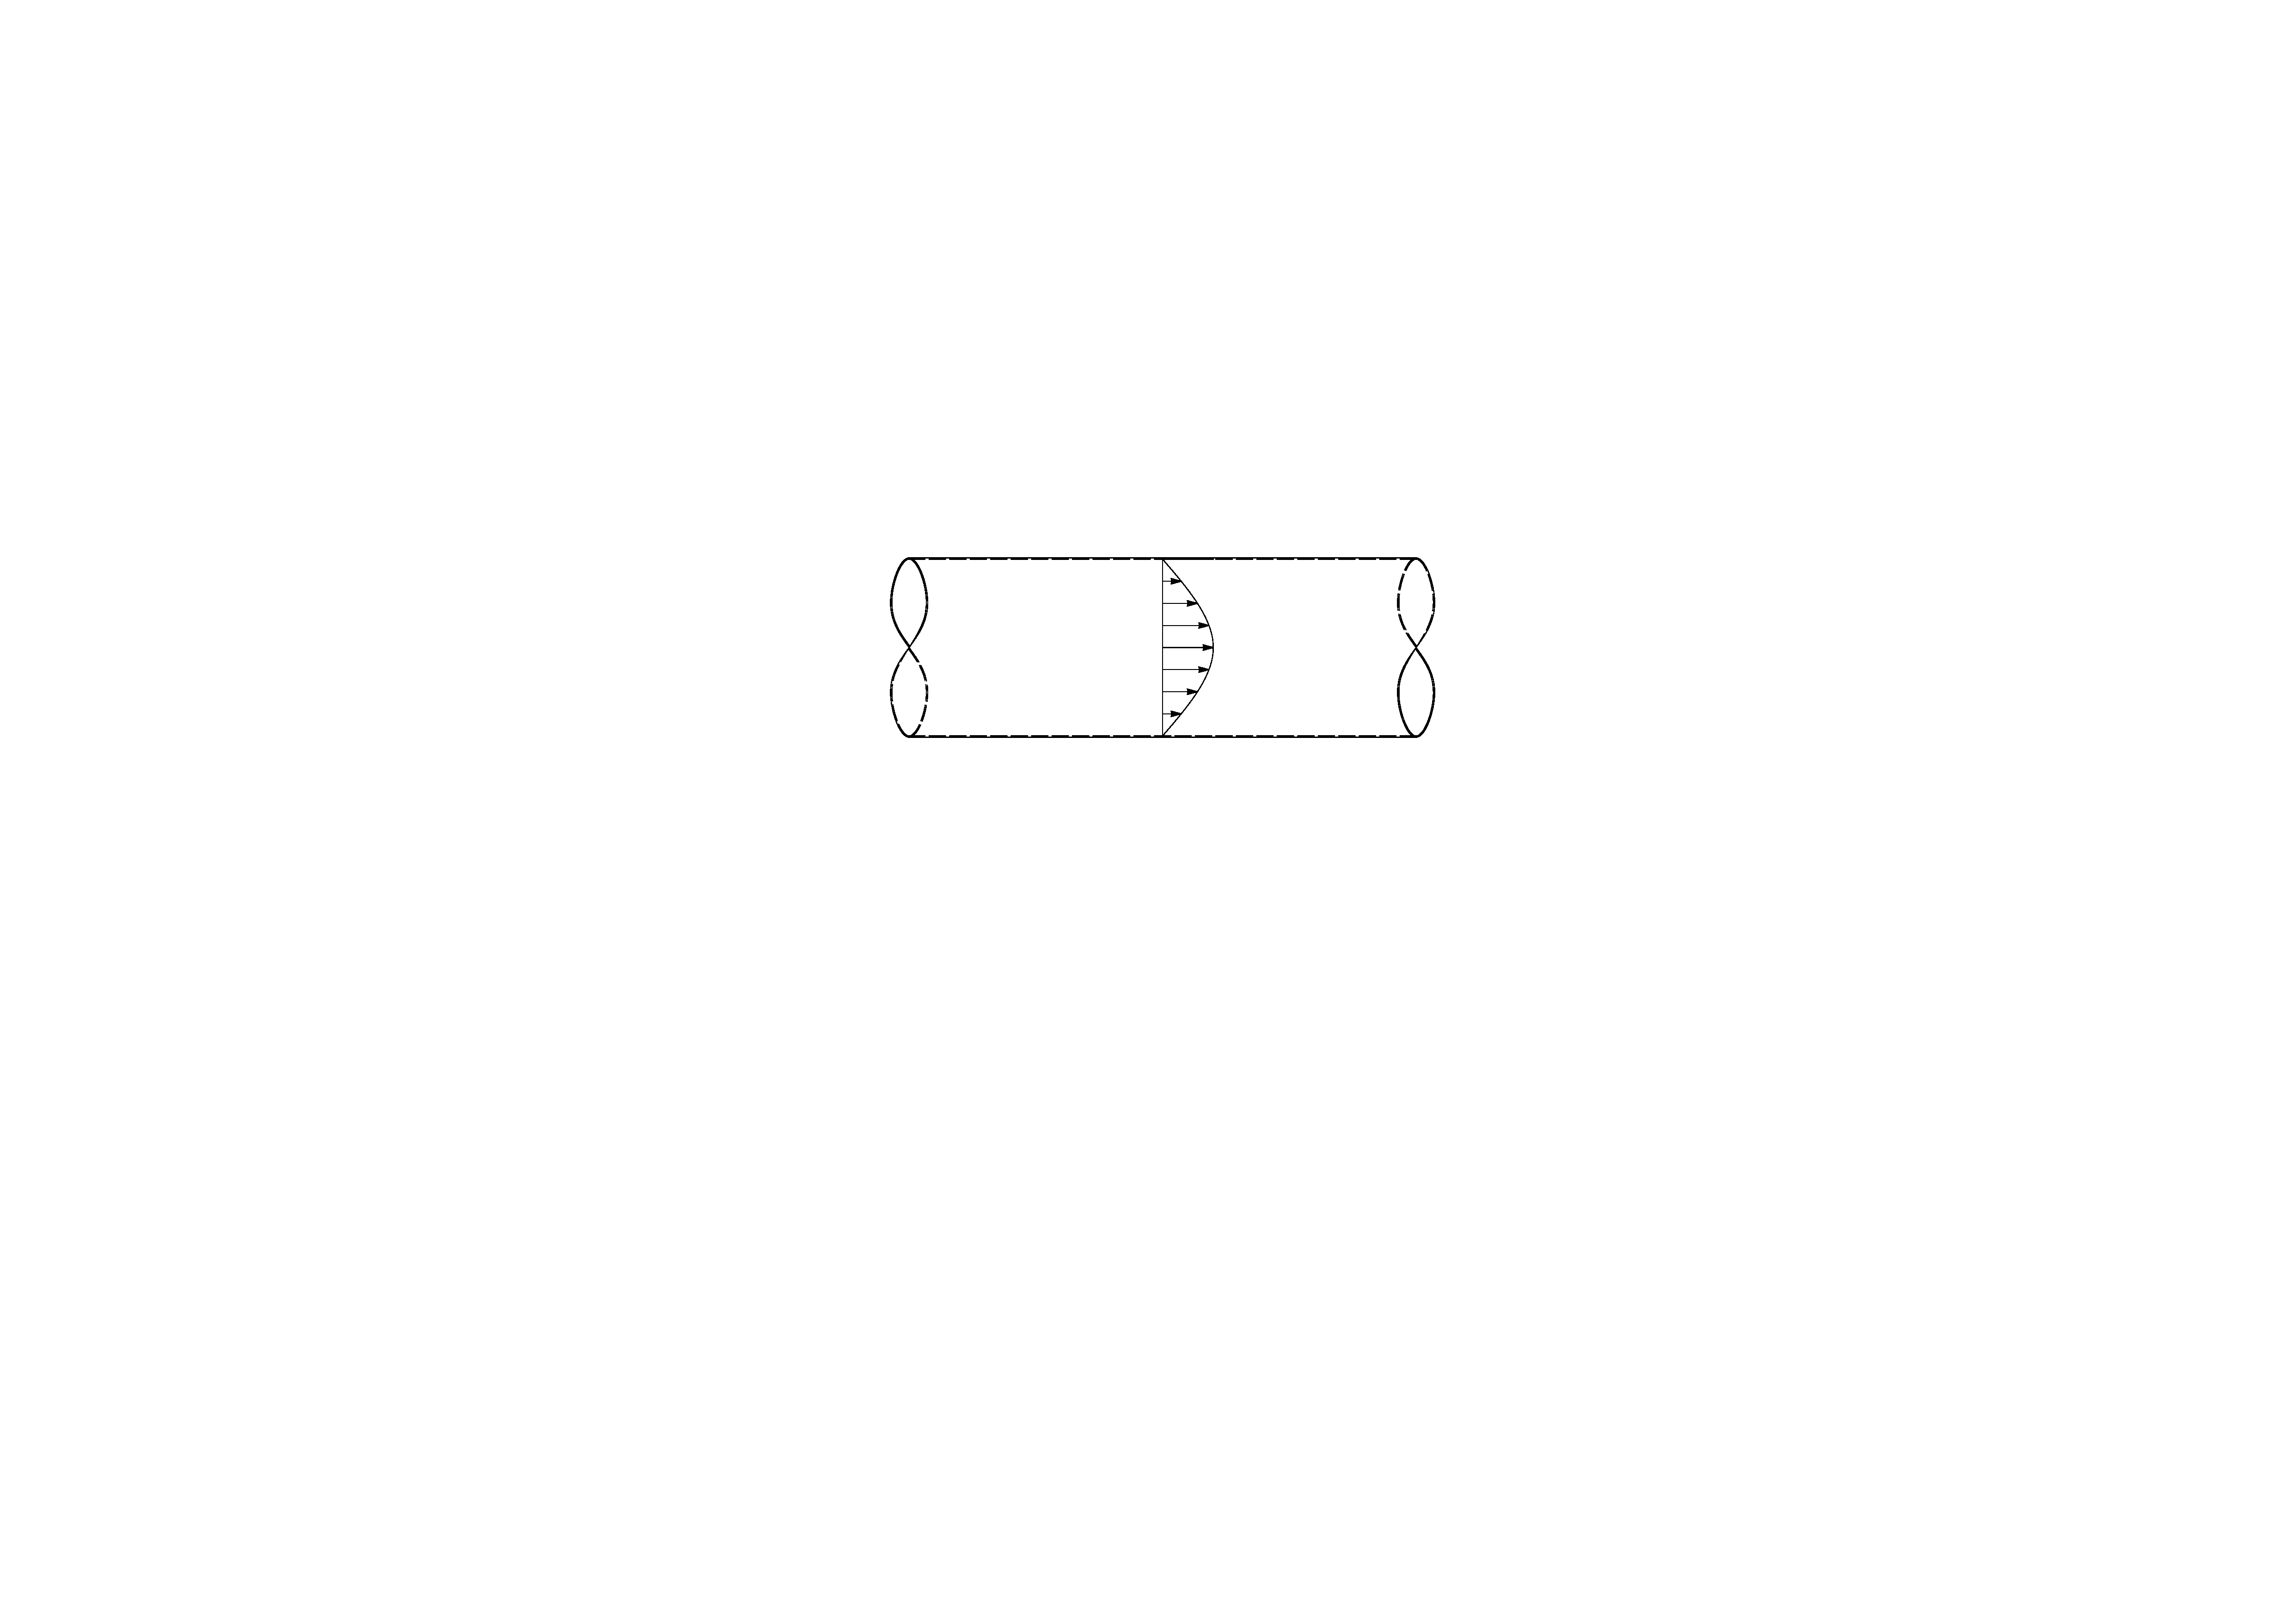
\includegraphics[width=.75\linewidth]{Figuras/EscLaminar.pdf}
        \caption{Escoamento laminar.}
        \label{fig:EscLaminar}
      \end{subfigure}
      \begin{subfigure}{.45\textwidth}
        \centering
        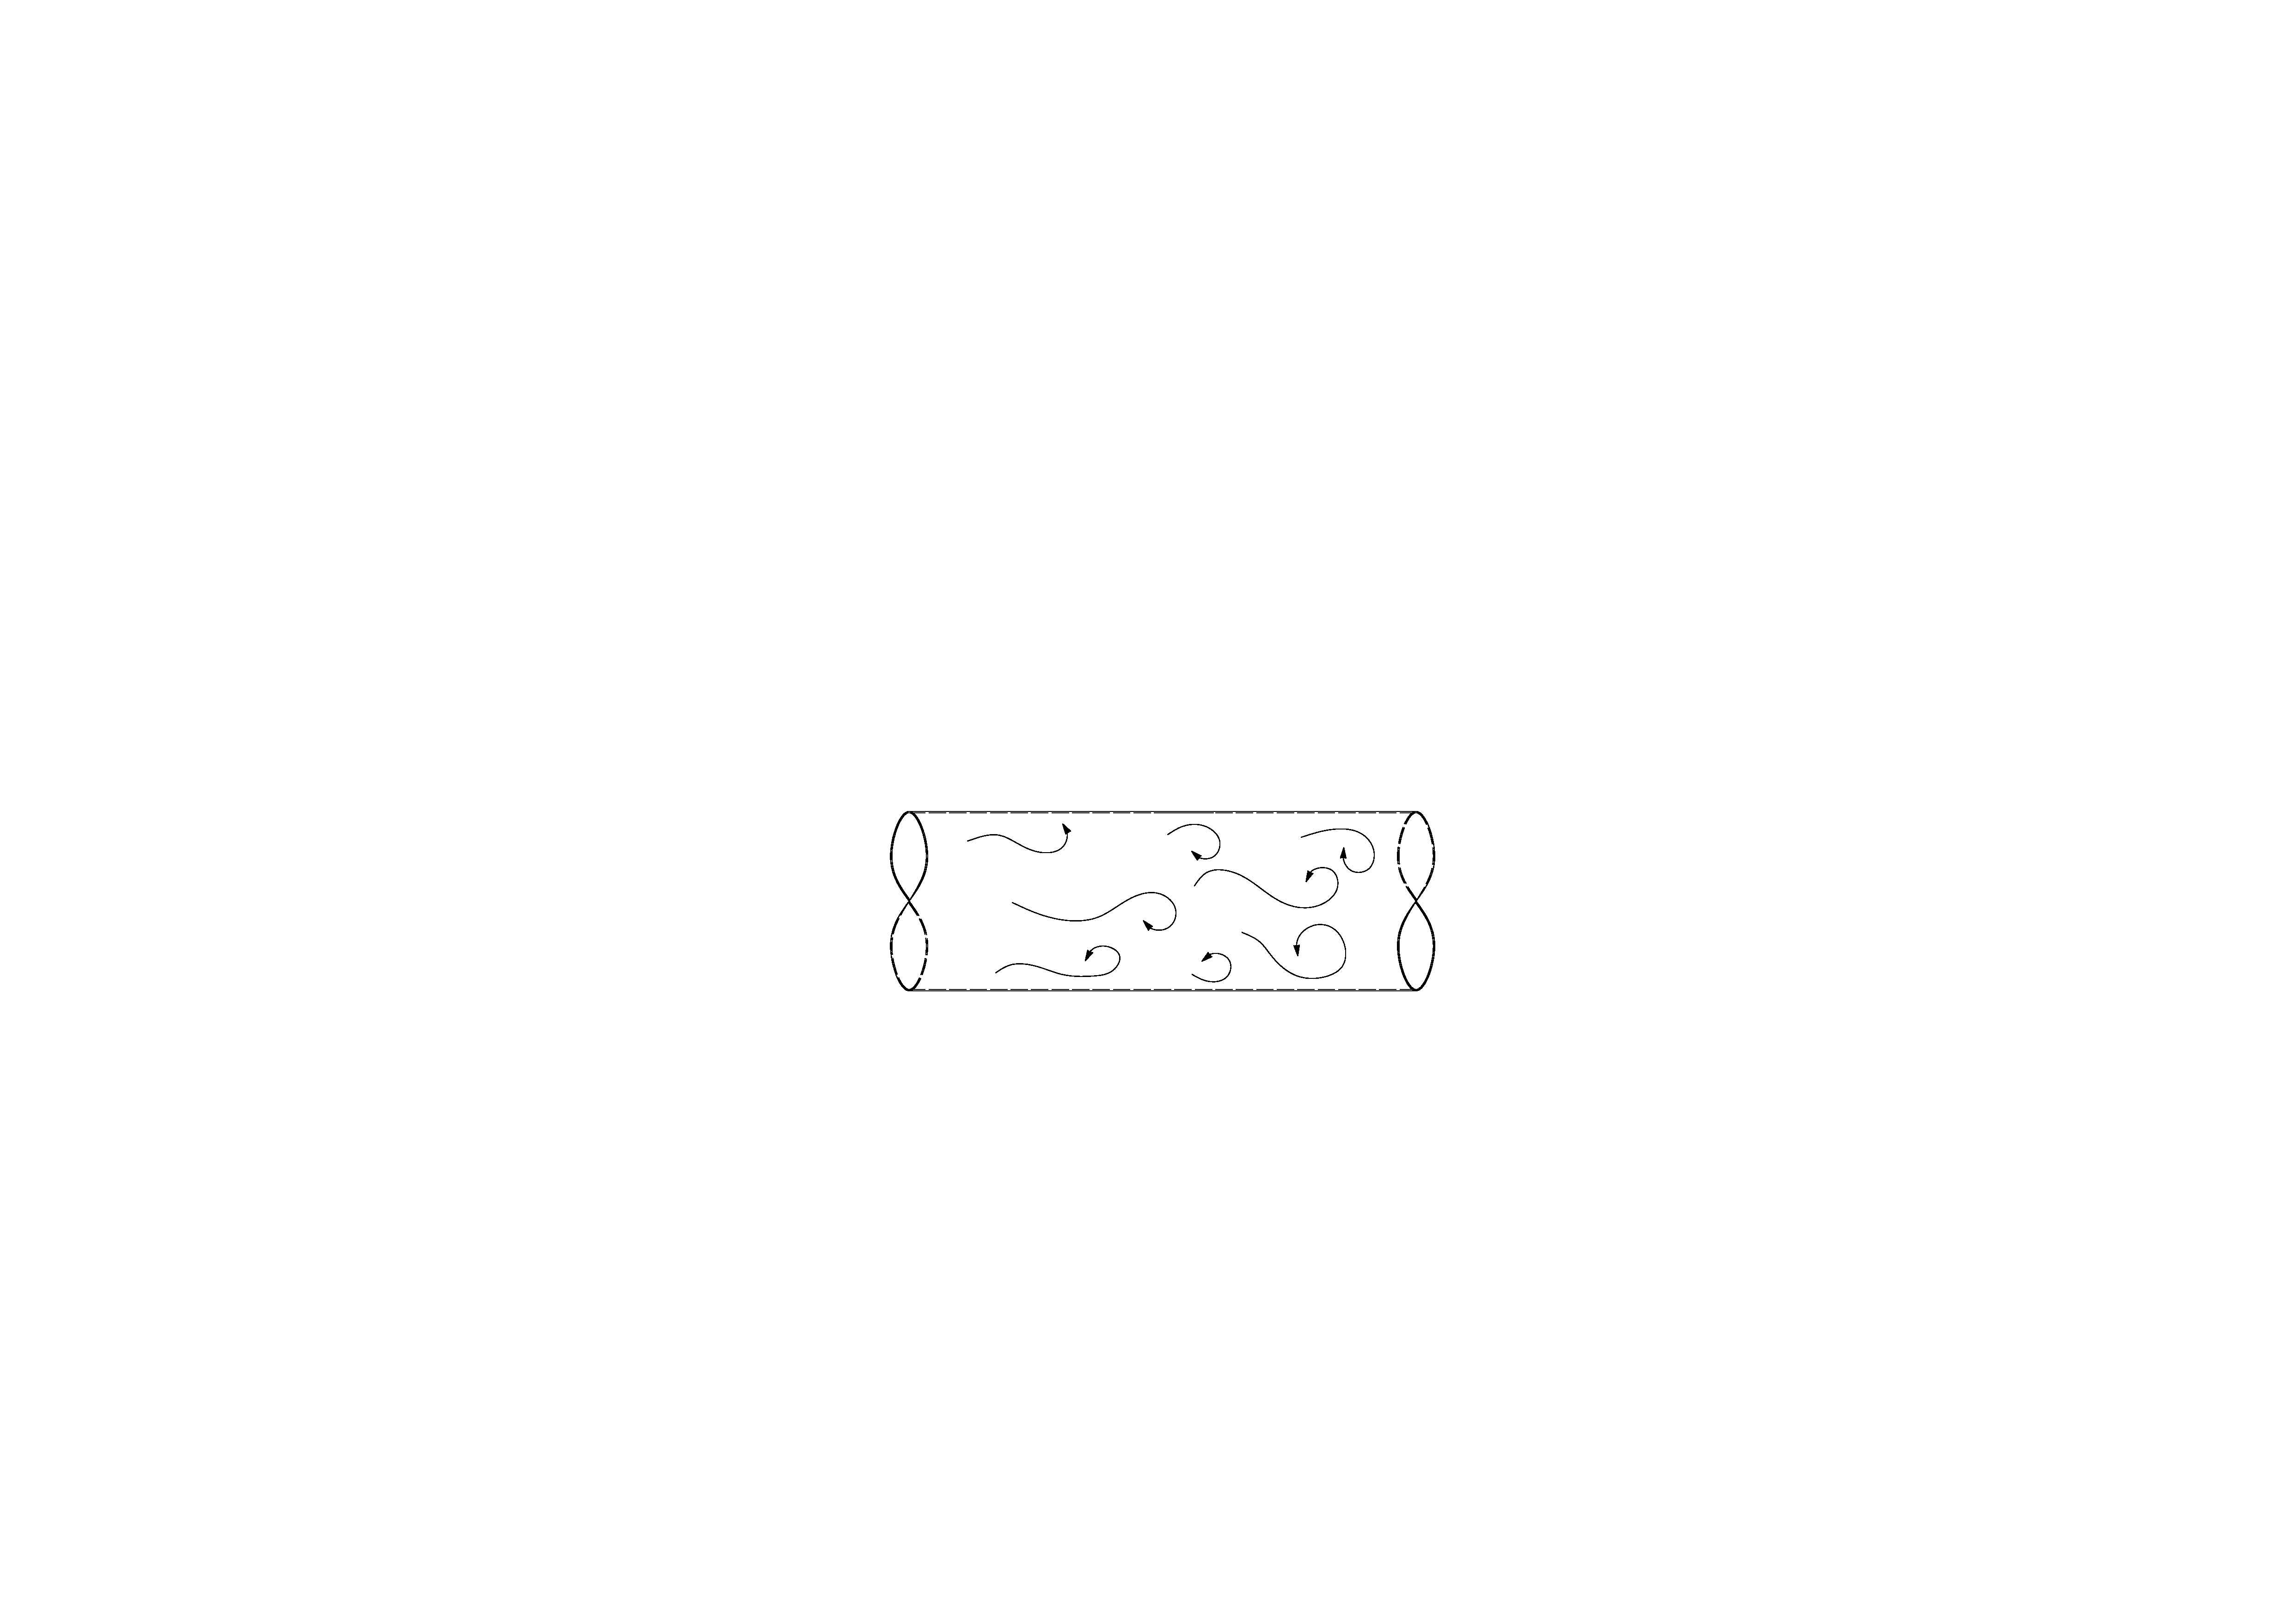
\includegraphics[width=.75\linewidth]{Figuras/EscTurbulento.pdf}
        \caption{Escoamento turbulento.}
        \label{fig:EscTurbulento}
      \end{subfigure}
    \\Fonte: Autoria Própria (\the\year).
\end{figure}

\end{document}